\section{Specifications}
\newcounter{rulei}[subsection]
\newcommand{\rcnii}{\stepcounter{rulei}\arabic{section}.\arabic{subsection}.\arabic{rulei}}
\renewcommand{\labelenumi}{\rcnii}

\subsection{Arena}
\begin{enumerate}
\item The match arena floor is an 8m x 8m square.
 The tolerance of the two arena dimensions is $\pm0.25m$.
\item The floor of the arena is made of white plastic coated hardboard.
 White Gaffer tape will be in place over the joints between hardboard sheets.
\item The arena walls are $600\pm30mm$ high and are made of the same material as the arena floor.
\item The arena is encased in a scaffolding structure, which is $1.4m \pm0.1m$ tall.
\end{enumerate}

\subsection{Tokens}
\label{tokens}
\begin {enumerate} 
\item Tokens will be cubes of side 45mm, to an accuracy of $\pm5mm$.
 Each team's kit contains a small number of these.
\item Tokens will weigh between WEIGHT and WEIGHT.
\item A token only accounts to a team's score when it is successfully placed in a zone.
 The token must be touching the zone floor in order to count.
\item Robots should not intentionally damage or destroy tokens.
\item The following token colours will be used: red, blue, yellow and green.
\end {enumerate}

\subsection{Robot Flags}
\label{sec:flags}
All robots must have a flagpole so that two flags can be mounted upon it:
\begin{description}
\item[Team Flag] The team flag is to be designed and created by the team.
 The team flag allows the robot to be easily identified.
 This flag must be mounted between 700mm and 900mm off the ground.
 It must not extend more than 200mm from the flagpole.

The team flag must not sag below 700mm above the ground.
\item[Match Flag] The match flag is to be supplied by Student Robotics at the start of every match.
 The match flag will slot over the top 100mm of the flagpole.
 The top 100mm of the flagpole must have an external diameter of $5\pm1$mm so that the match flag can slot over it.
 The match flags have an end-cap so that they will not slide down the flagpole.
\end{description}

The flagpole must be removable so that the robot can be placed within a box to check the size limit.
A diagram of the flagpole arrangement can be found in figure~\ref{fig:flag}.

\begin{figure}
\begin{center}
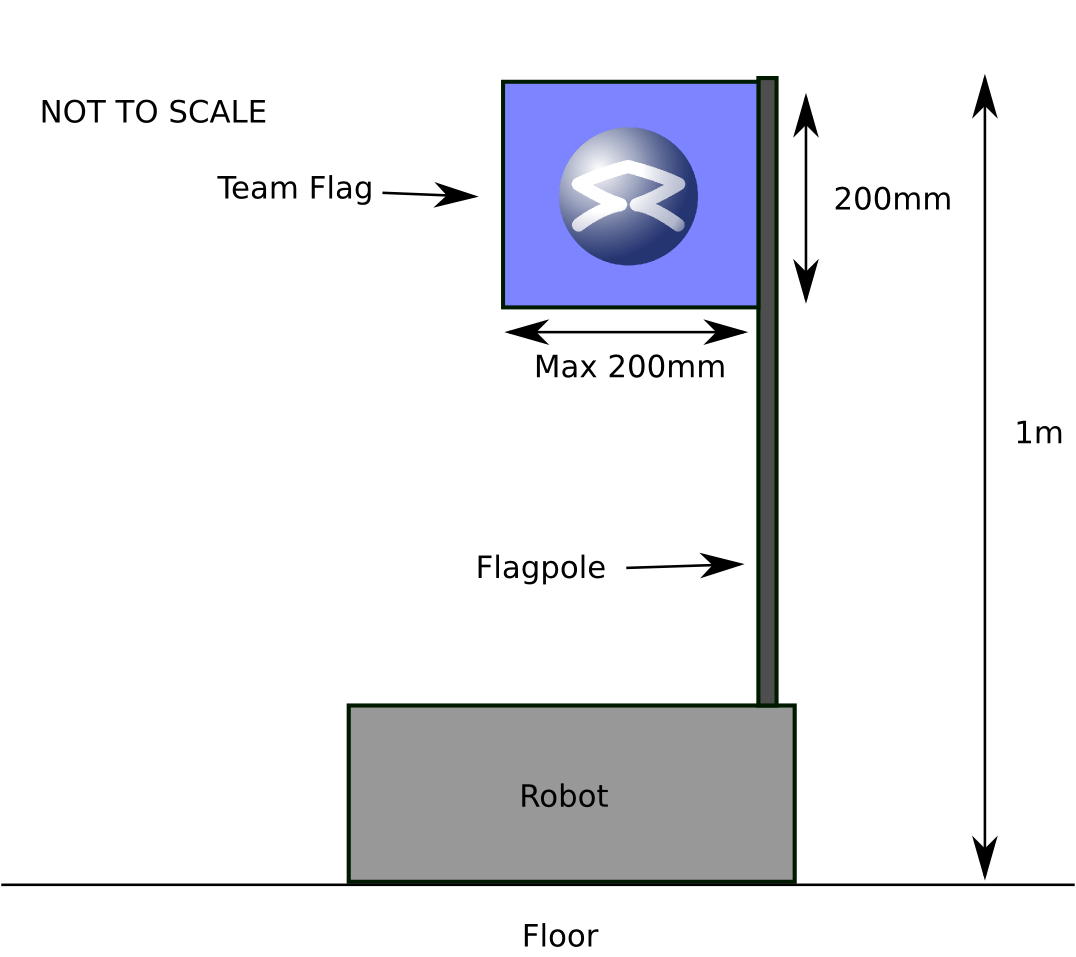
\includegraphics[keepaspectratio, scale =1]{./images/flag.png}
\caption{\label{fig:flag}Flagpole Dimensions}
\end{center}
\end{figure}
\clearpage
